\section{诱导引力波}

这一小节首先给出诱导引力波的计算公式,然后利用4.2节得到的原初功率谱给出数值结果。将发现计算得到的引力波的能量谱超出了LISA的灵敏度曲线,暗示LISA有可能观测到相应的引力波信号。最后针对幂函数形式的原初功率谱作一定的推广。

\subsection{基本方程}
从共性牛顿规范出发,扰动度规为如下形式
\begin{equation}
  \label{eq:second-order-perturbation-metric}
  ds^2=a^2(\eta) \left\{ -(1+2\Psi)d\eta^2+{\left[(1-2\Phi)\delta_{ij}+\frac{1}{2}h_{ij}\right]}dx^{i}dx^{j} \right\}.
\end{equation}
其中$\Psi$为一阶标量扰动,$h_{ij}$为二阶张量扰动,并且忽略了一阶张量扰动,矢量扰动和各项异性应力\citep{baumann2007gravitational}。

将二阶张量扰动作傅立叶变换得到
\begin{equation}
  \label{eq:second-tensor-perturbation-in-fourier-space}
  h_{ij}(\eta, \vec{x}) = \int \frac{d^3 \vec{k}}{{\left(2\pi \right)}^{3
  /2}} e^{i \vec{k}\cdot \vec{x}}
  {\left[h^{+}_{\vec{k}}(\eta)\mathrm{e}^{+}_{ij}(\vec{k})
  +h^{\times}_{\vec{k}}(\eta)\mathrm{e}^{\times}_{ij}(\vec{k})\right]},
\end{equation}
其中$\mathrm{e}^{+}_{ij}(\vec{k})$和$\mathrm{e}^{\times}_{ij}(\vec{k})$为极化张量,满足正交条件$\sum_{i,j}
\mathrm{e}^{\alpha}_{ij}(\vec{k})\mathrm{e}^{\beta}_{ij}(-\vec{k})=\delta^{\alpha\beta}$。后文中将极化指标。

从爱因斯坦方程出发,考虑扰动到二阶,可以推导出张量扰动模式在动量空间中满足的运动方程为
\begin{equation}
  \label{eq:equation-of-motion-for-second-tensor-perturbation}
  h^{\dprime}_{\vec{k}} +
  2\mathcal{H}h^{\prime}_{\vec{k}}+k^2h_{\vec{k}}=S(\eta,\vec{k}),
\end{equation}
其中$S(\eta,\vec{k})$是源项$S_{ij}(\eta,\vec{x})$的傅立叶变换,
\begin{equation}
  \label{eq:source-term-in-fourier-space}
  S(\eta, \vec{k}) = -4\mathrm{e}^{ij}(\vec{k}) \int
  \frac{d^3 \vec{x}}{{\left(2\pi \right)}^{3 /2}} e^{-i \vec{k}\cdot \vec{x}}
  S_{ij}(\eta, \vec{x}).
\end{equation}
源项的具体形式为\citep{ananda2007cosmological,baumann2007gravitational}
\begin{equation}
  \label{eq:source-term-in-real-space}
  S_{ij}(\eta, \vec{x}) = 
  4\Psi \partial_{i} \partial_{j} \Psi + 2\partial_{i} \Psi\partial_{j}
  \Psi - \frac{4}{3(1+w)\mathcal{H}^2}\partial_{i}
  (\Psi^\prime+\mathcal{H}\Psi)\partial_{j} (\Psi^\prime+\mathcal{H}\Psi). 
\end{equation}
运动方程$(\ref{eq:equation-of-motion-for-second-tensor-perturbation})$存在解析解,利用格林函数方法得到解析解为
\begin{equation}
  \label{eq:analytic-solution-of-equation-of-motion-for-second-tensor-perturbation} 
  h_{\vec{k}}(\eta)=\frac{1}{a(\eta)} \int^{\eta} d
  \tilde{\eta}G_{k}(\eta;\tilde{\eta}) \left[
  a(\tilde{\eta})S(\tilde{\eta}, \vec{k}) \right] ,
\end{equation}
其中$G_{k}(\eta;\tilde{\eta})$是如下方程的解
\begin{equation}
  \frac{d^2G_{k}(\eta;\tilde{\eta})}{d \tilde{\eta}^2} + \left(
  k^2-\frac{d^2 a}{ad \tilde{\eta}^2} G_{k}(\eta;\tilde{\eta}) \right) 
 = \delta(\eta-\tilde{\eta}).
\end{equation}
根据式$(\ref{eq:analytic-solution-of-equation-of-motion-for-second-tensor-perturbation})$只要求出源项$S(\tilde{\eta},
\vec{k})$,便能得到张量扰动的$\vec{k}$模式随时间的演化。为了解出源项,需要求解标量扰动的运动方程\citep{kodama1984cosmological,mukhanov1992theory}
\begin{equation}
  \label{eq:equation-for-scalar-perturbation}
  \Psi^{\dprime}_{\vec{k}}(\eta) +
  \frac{6(1+w)}{(1+3w)\eta}\Psi^\prime_{\vec{k}}(\eta) +
  wk^2\Psi_{\vec{k}}(\eta) = 0, 
\end{equation}
将$\Psi_{\vec{k}}(\eta)$拆分为两部分,初值$\psi_{\vec{k}}$以及与方向无关的转移函数$\Psi(k\eta)$
\begin{equation}
  \Psi_{\vec{k}}(\eta) \equiv \Psi(k\eta)\psi_{\vec{k}}. 
\end{equation}
于是源项的傅立叶变换可以改写为如下形式
\begin{equation}
  \label{eq:new-source-term-in-fourier-space}
  S(\eta, \vec{k}) = \int \frac{d^3 \vec{p}}{{\left(2\pi \right)}^{3 /2}} 
  \mathrm{e}(\vec{k}, \vec{p})f(\eta, \vec{k}, \vec{p})
  \psi_{\vec{k}}\psi_{\vec{k}-\vec{p}},
\end{equation}
其中
\begin{equation}
  \mathrm{e}(\vec{k},\vec{p}) = \mathrm{e}^{ij}(\vec{k})p_{i}p_{j},
\end{equation}
以及
\begin{equation}
  \begin{split}
    f(\eta, \vec{k}, \vec{p}) = & \frac{8(3w+5)}{3(w+1)}
    \Psi(\lvert \vec{p}\rvert\eta)\Psi(\lvert \vec{k}-\vec{p}\rvert\eta) +
    \frac{4{\left(3w+1\right)}^2}{3(w+1)}\eta^2 \Psi^\prime(\lvert
    \vec{p}\rvert\eta) \psi^\prime(\lvert \vec{k}-\vec{p}\rvert\eta) \\
    & + \frac{8(3w+1)}{3(w+1)}\eta 
    \left[ \psi^\prime(\lvert \vec{p}\rvert \eta)\psi(\lvert
    \vec{k}-\vec{p}\rvert\eta)+\psi(\lvert
    \vec{p}\rvert\eta)\Psi^\prime(\lvert \vec{k}-\vec{p}\rvert\eta) \right].
  \end{split}
\end{equation}
对于视界内的模式而言,引力波的能量谱可以用引力波的功率谱来表示
\begin{equation}
  \label{eq:energy-spectrum-for-GW-in-power-spectrum}
  \Omega_{GW}(\eta, k) \equiv \frac{1}{\rho_{c}} \frac{d\rho_{GW}}{d \ln k}
  = \frac{1}{24} {\left(\frac{k}{\mathcal{H}}\right)}^2
  \overline{\mathcal{P}_{h}(\eta, k)},
\end{equation}
其中上划线代表取振荡平均,$\rho_{c}$为宇宙的临界能量密度,并且已经对两个极化模式进行了求和。引力波的功率谱$\mathcal{P}_{h}$定义为
\begin{equation}
  \label{eq:power-spectrum-definition-of-GW}
  \langle h_{\vec{k}}(\eta)h_{\vec{p}}(\eta)\rangle = \frac{2\pi^2}{k^3} 
  \delta^3(\vec{k}+\vec{p})\mathcal{P}_{h}(\eta, k).
\end{equation}
为了计算张量扰动在动量空间的两点关联函数,利用式$(\ref{eq:analytic-solution-of-equation-of-motion-for-second-tensor-perturbation})$和$(\ref{eq:new-source-term-in-fourier-space})$得到
\begin{equation}
  \langle h_{\vec{k}}(\eta)h_{\vec{p}}(\eta)\rangle = \int
  \frac{d^3q d^3 \tilde{q}}{{\left(2\pi^3\right)}^3}
  \mathrm{e}(\vec{k},\vec{p})\mathrm{e}(\vec{p}, \tilde{\vec{q}})
  I(\eta, \vec{k},\vec{q})I(\eta, \vec{p}, \tilde{\vec{q}})
  \langle
  \psi_{\vec{q}}\psi_{\vec{k}-\vec{q}}\psi_{\tilde{\vec{q}}}\psi_{\vec{p}-\tilde{\vec{q}}}\rangle,
\end{equation}
其中
\begin{equation}
  I(\eta, \vec{k},\vec{p}) \equiv \int^{\eta} d \tilde{\eta}
  \frac{a(\tilde{\eta})}{a(\eta)} G_{k}(\eta;\tilde{\eta})f(\tilde{\eta},
  \vec{k}, \vec{p}).  
\end{equation}

$\psi_{\vec{k}}$为$\vec{k}$方向的初始随机涨落。假设所有方向互相独立且都服从相同的高斯分布,
那么根据Wick定理,$\psi_{\vec{k}}$的四点关联函数能够转化为两点关联函数。引入无
量纲变量$u\equiv\lvert \vec{k}-\vec{p}\rvert /k$、$v\equiv \lvert
\vec{p}\rvert /k$以及$x\equiv k\eta$后,获得张量扰动功率谱的最终形式
\begin{equation}
  \label{eq:last-result-for-power-spectrum-of-second-tensor-perturbation}
  \mathcal{P}_{h}(\eta, k) = 4 \int_{0}^{\infty} \int_{\lvert
  1-v\rvert}^{1+v} du
  {\left(\frac{4v^2-{\left(1+v^2-u^2\right)}^2}{4uv}\right)}^2
  \mathcal{I}^2(x, u, v)\mathcal{P}_{\mathcal{R}}(ku)
  \mathcal{P}_{\mathcal{R}}(kv),  
\end{equation}
其中
\begin{equation}
  \label{eq:integral-function}
  \mathcal{I}(x, u,v) \equiv I(\eta, \vec{k}, \vec{p})k^2. 
\end{equation}

进行到这一步,我们已经把曲率扰动功率谱和二阶张量扰动的功率谱联系了起来。剩下的
问题变成求解曲率扰动功率谱和如何求积分。

对于4.2小节中由双拐点暴胀得到的标量扰动功率谱,尖峰对应的模式是在辐射为主时期进入的视界,因此当时的物态参数为$w=1
/3$,方程$(\ref{eq:equation-for-scalar-perturbation})$的解可以简化到
\begin{equation}
  \label{eq:solution-for-scalar-perturbation-in-radiation-era}
  \Psi(x) = \frac{9}{x^2}{\left(\frac{\sin(x /\sqrt{3})}{x/ \sqrt{3}}
  -\cos(x /\sqrt{3})\right)},
\end{equation}
以及格林函数
\begin{equation}
  \label{eq:green-function-in-radiation-era}
  G_{k}(\eta;\tilde{\eta}) = \frac{\sin(k\eta-k \tilde{\eta})}{k}.
\end{equation}
标量功率谱中尖峰对应的尺度为$10^{13}\text{Mpc}^{-1}$,相比与基准尺度$k_{\star}=0.05\text{Mpc}^{-1}$\citep{akrami2018planck}大出很多个量级。
从标量扰动在辐射为主时期的解$(\ref{eq:solution-for-scalar-perturbation-in-radiation-era})$能够看出,扰动进入视界的时间越长,扰动大小被压低的越厉害。因此诱导引力波的产生主要是在对应的模式刚好进入视界的那一小段时间之内。这个性质允许我们
采用文章\citep{kohri2018semianalytic}中应用的方法,在进入视界并经过较长的时间后取振荡平均作为结果,即
\begin{equation}
  \label{eq:oscillation-average-after-entering-horizon}
  \begin{split}
    &\overline{\mathcal{I}^2(x\rightarrow \infty,u,v)} = 
    \frac{1}{2}{\left(\frac{3}{4u^3v^3x}\right)}^2{\left(u^2+v^2-3\right)}^2
    \\
    &{\left({\left[-4uv+(u^2+v^2-3)\ln \left\lvert
      \frac{3-{\left(u+v\right)}^2}{3-{\left(u-v\right)}^2}\right\rvert\right]}^2+{\left[\pi
     (u^2+v^2-3)\Theta(u+v-\sqrt{3}) \right]}^2\right)},
  \end{split}
\end{equation}
其中$\Theta$为Heaviside
theta函数。联合式$(\ref{eq:power-spectrum-definition-of-GW})$和$(\ref{eq:integral-function})$,
以及辐射为主时期有$\mathcal{H}=1 /\eta$,得到了引力波能量谱的最终表达式
\begin{equation}
  \label{eq:final-energy-spectrum-of-GW} 
  \begin{split}
    \Omega_{GW}(\eta, k) &= \frac{1}{12} \int_{x=0}^{\infty}dv \int_{\lvert
    1-v\rvert}^{1+v} du
    {\left(\frac{4v^2-{\left(1+v^2-u^2\right)}^2}{4uv}\right)}^2
    \mathcal{P}_{\mathcal{R}}(ku) \mathcal{P}_{R}(kv) \\
    & {\left(\frac{3}{4u^3v^3}\right)}^2 {\left(u^2+v^2-3\right)}^2 \\
    &{\left(
    {\left[-4uv+(u^2+v^2-3)\ln \left\lvert
\frac{3-{\left(u+v\right)}^2}{3-{\left(u-v\right)}^2}\right\rvert\right]}^2
+ {\left[\pi (u^2+v^2-3)\Theta(u+v- \sqrt{3})\right]}^2\right)}.
  \end{split}
\end{equation}

\subsection{数值结果}
上一小节得到了双拐点暴胀模型中诱导引力波的数值结果。为了与LISA\citep{amaro2017laser}和太极(Taiji)\citep{guo2018taiji}的灵敏度曲线进行比较,
将在辐射为主时期产生的引力波能量谱换算到现在时刻,用$\Omega_{\text{GW},0}$表示
\begin{equation}
  \label{eq:energy-spectrum-of-GW-at-now}
  \Omega_{\text{GW},0} =
  \Omega_{r,0}{\left(\frac{g_{*,0}}{g_{*,p}}\right)}^{1
  /3}\Omega_{\text{GW}},
\end{equation}
其中$\Omega_{r,0}$是当前时刻辐射密度占总能量密度的比重,$g_{*,0}$和$g_{*,p}$是当前时刻以及标量功率谱尖峰进入视界时的相对论有效自由度的数目。因为灵敏度曲线的横轴是频率,因此还需要波数$k$与频率$f$之间的变换关系
\begin{equation}
  \label{eq:frequency-from-wave-numbers}
  f \approx 0.03\text{Hz} \frac{k}{2\times 10^{7}\text{pc}^{-1}}.
\end{equation}
从图$(\ref{fig:curve-for-induced-gw-and-LISA-and-Taiji})$我们可以看到诱导引力波能量谱的数值结果位于LISA\citep{amaro2017laser}和Taiji\citep{guo2018taiji}的期望灵敏度曲线之上。
与LISA相比,Taiji的灵敏度曲线向低频方向有所偏移,这与Taiji的观测设备之间相隔距离更大有关。
模型预言的峰值频率大约为$0.05\text{Hz}$,落在空基引力波探测器的探测频段范围内,意味着如果存在,那么诱导引力波信号理论上能够被LISA和Taiji观测到。

尖峰对应的模式用$k_{p}$表示。通过数值拟合发现,在$k_{p}$两侧区域,引力波能量谱
$\Omega_{\text{GW}}$基本上能由模式$k$的幂函数来表示。在$k\ll
k_{p}$的区域,$\Omega_{\text{GW}}\approx
k^3$。这与由预加热和相变作为源产生的随机引力波背景具有相同的结果,不过在$k\gg
k_{p}$区域,我们的模型给出了不同于其它引力波源的幂指标$1.9$。

\begin{figure}[!htbp]
  \centering
  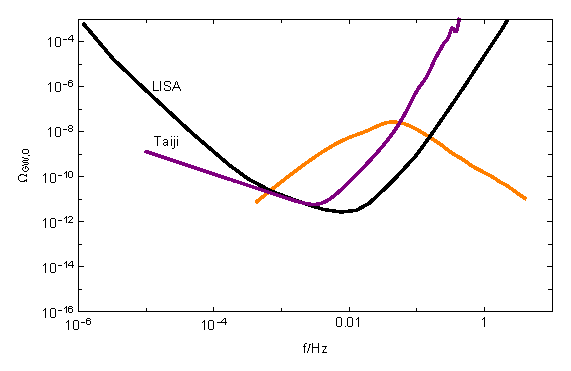
\includegraphics[width=6in]{Img/Lisa2.eps}
  \caption{橙色实线为双拐点暴胀模型预言的诱导引力波的能量谱曲线。黑/红色曲线分别是LISA\citep{amaro2017laser}和太极(Taiji)\citep{guo2018taiji}的期望灵敏度曲线。}\label{fig:curve-for-induced-gw-and-LISA-and-Taiji}
\end{figure}

\subsection{幂函数功率谱的情况}
正如图$(\ref{fig:pert})$中所示,原初功率谱在尖峰附近能够近似由模式$k$的幂函数来表示。
\begin{equation}
  \mathcal{P}_{\mathcal{R}}(k) \approx
  \begin{cases}
    k^{n_1},  \qquad k \ll k_{p} \\
    k^{n_2}, \qquad k \gg k_{p}
  \end{cases}
\end{equation}

在这种情况下,引力波的能量谱也能通过分段幂函数来表示,
\begin{equation}
  \Omega_{\text{GW}}(k) \approx
  \begin{cases}
    k^{m_1}, \qquad k \ll k_{p} \\
    k^{m_2}, \qquad k\gg k_{p}
  \end{cases}
\end{equation}
幂指标$m_1$和$m_2$分别为$n_1$和$n_2$的函数。先讨论$k\ll
k_{p}$的情况,因为$v$和$u$反比于$k$,式$(\ref{eq:final-energy-spectrum-of-GW})$积分的主要贡献来自于区域$1\ll
v,u\le k_{p}
/k$,因此对$\Omega_{\text{GW}}$的主要贡献来自于尖峰附近。在这一近似下,式$(\ref{eq:final-energy-spectrum-of-GW})$
简化为
\begin{equation}
  \Omega_{\text{GW}}(k) \propto k^{2n_1} \int_{0}^{k_{p} /k} dv v^{2n_1-4}.
\end{equation}
若$n_1 > 2$,积分体在区间$ \left[ 0,\ k_{p}/k \right]$内有限,结果为
\begin{equation}
  \Omega_{\text{GW}}(k) \propto k^3. 
\end{equation}
再考虑$k\gg k_{p}$的情况。当满足条件$v\ll 1$或$u\ll
1$时,积分体简化为$v^{3-n_2}$。又当$n_2 >
-4$时,式$(\ref{eq:final-energy-spectrum-of-GW})$可以表示成
\begin{equation}
  \label{eq:energy-spectrum-for-k-larger-than-kp}
  \Omega_{\text{GW}}(k) \propto k^{2n_2} \int_{-\infty}^{\infty} dv F(v).  
\end{equation}
由于式$(\ref{eq:energy-spectrum-for-k-larger-than-kp})$中积分部分与$k$无关,因此$\Omega_{\text{GW}}(k)
\propto k^{2n_2}$。而当$n_2\le
-4$时,式$(\ref{eq:final-energy-spectrum-of-GW})$中积分的主要贡献来自于区间
$k_{p}/k \le v\ll 1$或者$k_{p}/k \le u\ll 1$,因此能够化简为
\begin{equation}
  \Omega_{\text{GW}}(k) \propto k^{2n_2} \int_{k_{p}/k}^{\epsilon} dv
  v^{3-n_2},   
\end{equation}
其中$\epsilon$满足条件$k_{p}/k\ll \epsilon\ll 1$。因此积分结果又有两种情况
\begin{equation}
  \Omega_{\text{GW}}(k) \propto
  \begin{cases}
    k^{n_2-4} , \qquad & n < -4 \\
    k^{n_2-4}\ln (k_{p}/k), \qquad & n_2= -4
  \end{cases}.
\end{equation}

\begin{figure*}
  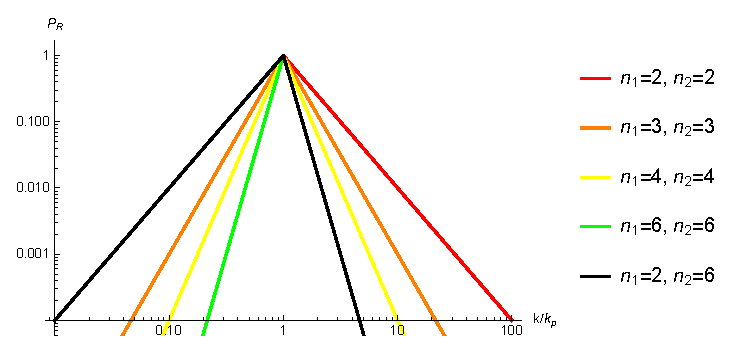
\includegraphics[width=3in]{Img/PR.eps}
  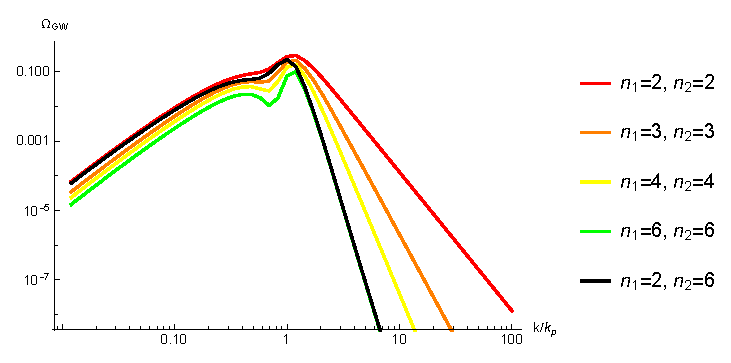
\includegraphics[width=3in]{Img/omega.eps}
  \caption{$\Omega_{\text{GW}}$关于变量$k$的渐进幂函数行为。左侧,给出了几个带有不同幂指标的$P_{\mathcal{R}}$的例子。右侧为对应的$\Omega_{\text{GW}}$的结果。}\label{fig:label}
\end{figure*}

